\section{Numerical Experiments}
In this section compare the accuracy of two-pass and one-pass fix rank approximation algorithms compared to the classical Tucker decomposition for both synthetic examples and real data. 

\subsection{Synthetic Examples} 
\subsubsection{Experimental Setup}
For simplicity, all numerical experiments with synthetic examples assume that $\mathscr{X}$ has equal side length, $I$. We consider two scenarios from the the view of signal recovery and approximation error respectively. In case of signal recovery, we set $\mathscr{X} = \mathscr{X}^\natural+\mathscr{E}$, where $\mathscr{X}^\natural$ is the low rank signal tensor and $\mathscr{E}$ is the Gaussian noise tensor. Then, we evaluate the relative error as $\left|\llbracket \hat{\mathscr{X}} \rrbracket_\mathbf{r} -  \mathscr{X}^\natural\|_F\right|/{\|\mathscr{X}^\natural\|_F}$, where $\llbracket \hat{\mathscr{X}} \rrbracket_\mathbf{r}$ is rank $\mathbf{r}$ approximation by the one-pass or two-pass fixed rank algorithm.

From the view of approximation error, we set $\mathscr{X}$ to be a super-diagonal tensor with decaying values along super-diagonal after $r$th entry. Under this scenario, we evaluate the algorithm accuracy by the relative error: $\left| \llbracket \hat{\mathscr{X}}\rrbracket_\mathbf{r} -  \mathscr{X} \|_F\right|/\|\mathscr{X}\|_F$,
where $\llbracket \hat{\mathscr{X}} \rrbracket_\mathbf{r}$ is the rank $\mathbf{r}$ approximation by our two algorithms. 

Now we present the details of our data-generating procedure. In the low rank plus noise case, we let $\gamma$ be the \textit{noise level}. Then, given a low rank tensor $\mathscr{X}^\natural\in \mathbb{R}^{I_1\times \dots \times I_N}$ as our true signal, we add a random noise tensor with each element from $\mathcal{N}(0, \sigma^2)$ where $\sigma^2 = \gamma^2 \|\mathscr{X}^\natural\|_F^2 / \bar{I}$ and $\bar{I} = \prod_{n=1}^N I_n$. Since $\|\mathscr{X}^\natural\|_F$ represents the true signal strength, the square of noise to signal ratio $\gamma^2 \approx \frac{\mathbb{E} \|E\|^2}{\|\mathscr{X}^\natural\|_F^2}= \frac{\sigma^2 \bar{I}}{\|\mathscr{X}^\natural\|_F^2}$. Additionally, given Corollary \ref{corollary:fix_rank_err}, we set $s = 2k+1$ in the one-pass algorithms.
\begin{enumerate}[topsep=0pt,itemsep=-1ex,partopsep=1ex,parsep=1ex]
    \item Superdiagonal + Noise: Superdiagonal tensor with rank $r$ + $\sqrt{\frac{\gamma^2 \cdot r}{I^N}} \mathcal{N}(0,1)$. we consider three settings with the noise level $\gamma = 0.01, 0.1, 1$ to represent the low noise, medium noise and high noise cases,
    \item Polynomial Decay: 
    \begin{equation}
        \mathscr{X} = \rm{superdiag}(1,\dots,1, 2^{-t},3^{-t},\dots, (N-r)^{-t}).
    \end{equation}
    We consider two cases where $t = 1,2$ representing slow and fast polynomial decay cases. 
    \item Exponential Decay: 
    \begin{equation}
        \mathscr{X} =  \rm{superdiag}(1,\dots,1, 10^{-t},10^{-2t},\dots, (10)^{-(N-r)t}) 
    \end{equation}
    We consider two cases where $t = 0.25,1$ representing slow and fast exponential decay. 
    \item Low Rank: Generate a core tensor $\mathscr{C} \in \mathbb{R}^{k \times \dots \times k}$, with each entries $\rm{Unif}([0,1])$. Independently generate $N$ orthogonal arm matrices by first creating $\mathbf{A}_1, \dots, \mathbf{A}_N$, with each entry $\mathcal{N}(0,1)$, and then computing the arm matrices by $(\mathbf{Q}_n, \sim) = \rm{QR}(\mathbf{A}_n)$, for $1 \leq n \leq N$.  
    \begin{equation}
        \mathscr{X} = \mathscr{C} \times_1 \mathbf{Q}_1 \times \cdots \times_N \mathbf{Q}_N + \sqrt{\frac{\gamma^2 \cdot \|\mathscr{X}^\sharp\|_F^2}{I^N}} \mathcal{N}(0,1).
    \end{equation}
\end{enumerate}

\subsubsection{Numerical Results} 
Figure \ref{fig:id_lnoise} and \ref{fig:more_result} display the performance for Tucker Decomposition, one pass and two pass fixed rank algorithm with different input tensors. In all cases with noisy input tensor with the noise level $\gamma$, Tucker decomposition performs very well with a relative error approximate to $\gamma$. The relative error for one-pass and one-pass algorithms converges to that of Tucker decomposition as $k$ increases. In particular, the convergence rate is higher when the noise is lower or $n$ is larger. In noiseless cases, we observe a similar pattern: the relative error for two-pass and one-pass algorithms converges to that of Tucker decomposition. In particular, the algorithm achieves convergence at relatively small $k$. The rate is higher when the decaying rate is higher. 

\begin{figure}[H] 
    \centering 
    \begin{subfigure}{0.32\textwidth}
    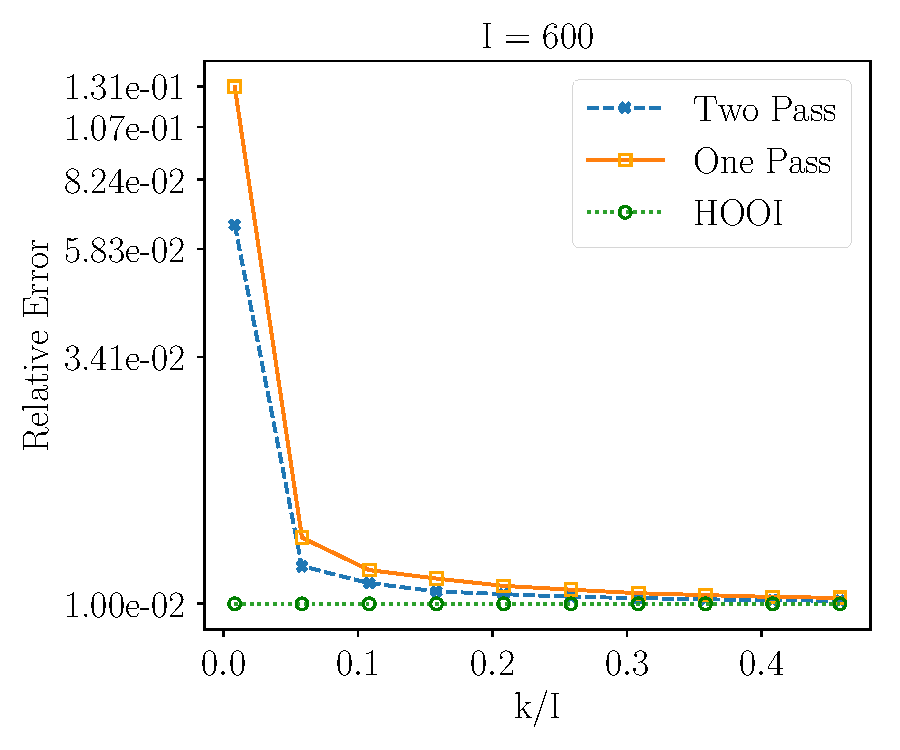
\includegraphics[scale = 0.3]{figure/id_lnoise_n600.pdf}
    \end{subfigure}
    \begin{subfigure}{0.32\textwidth}
    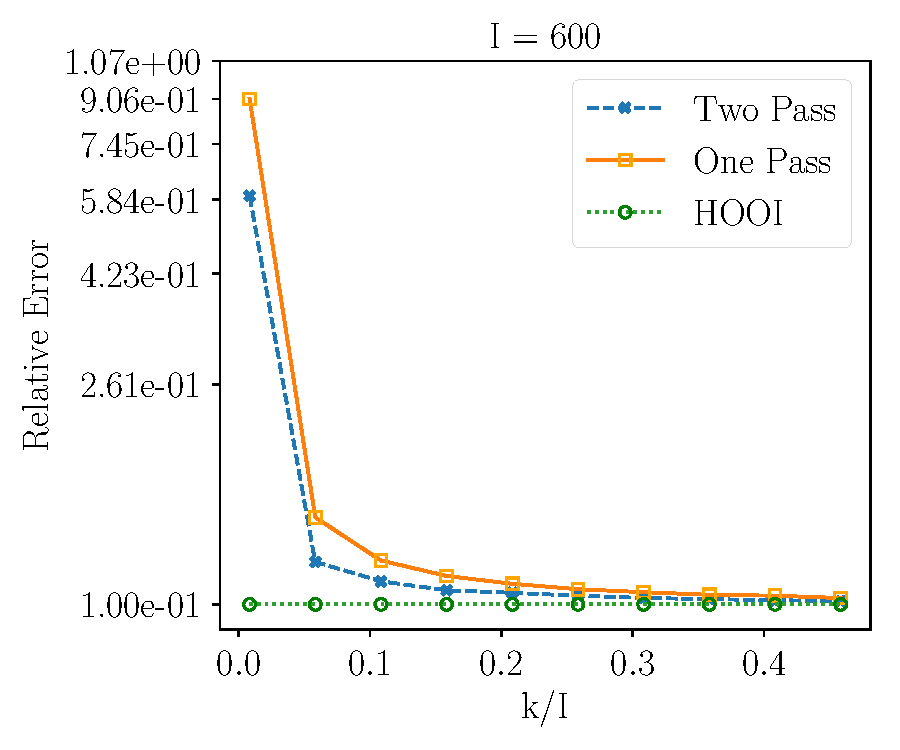
\includegraphics[scale = 0.3]{figure/id_mnoise_n600.pdf}
    \end{subfigure}
    \begin{subfigure}{0.32\textwidth}
    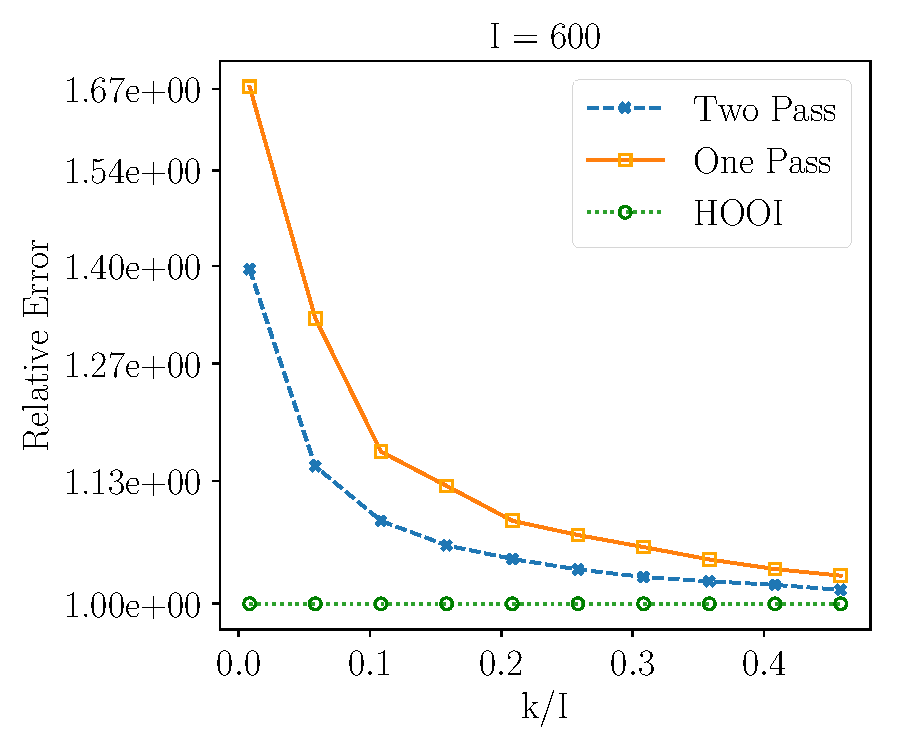
\includegraphics[scale = 0.3]{figure/id_hnoise_n600.pdf}
    \end{subfigure}
    \textbf{Superdiagonal +Low/Medium/High Noise ($\gamma = 0.01,0.1,1$)}
\caption{Relative error for fixed-rank tensor approximation as a function of the compression factor $k/n$: \textit{We compare the relative errors presented in log scale for two-pass sketching, one-pass sketching and Tucker decomposition for the input tensor with superdiagonal + noise design ($\gamma = 0.01,0.1,1$). Rank $r$ = 5.}} \label{fig:id_lnoise}
\end{figure}

\subsection{Application Examples}

For real-world application of our methods, we experimented on the state-of-the-art global climate simulation datasets based on the Community Earth System Model (CESM) Community Atmosphere Model (CAM) 5.0 \cite{hurrell2013community,kay2015community}. In particular, we used the dataset on aerosol absorption, which can affect climate through absorbing the solar radiation and changing cloud formation. This dataset recorded absorption at different times, altitudes, longitudes, and latitudes  ($240 \times 30 \times 192 \times 288$). Since the Tucker rank of the original tensor remains unknown, we compared different models for different choices of rank, with the result given in Figure \ref{fig:application}. Also, we performed additional experiments on the net surface radiative flux and dust aerosol burden data with the results given in Figure \ref{fig:srfrad}, \ref{fig:burden_dust} in Appendix \ref{appendix: more_real_data_result}. 
\begin{figure}[H] 
    \centering 
    \begin{subfigure}{0.31\textwidth}
    \end{subfigure}
    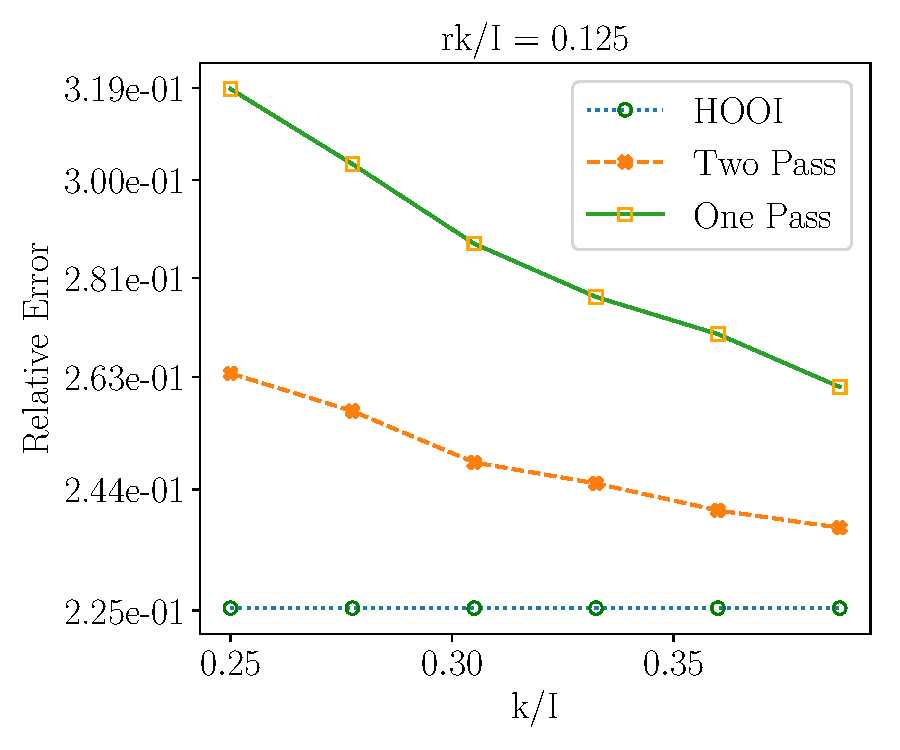
\includegraphics[scale = 0.29]{figure/ABSORB_frk8.pdf}
    \begin{subfigure}{0.31\textwidth}
    \end{subfigure}
    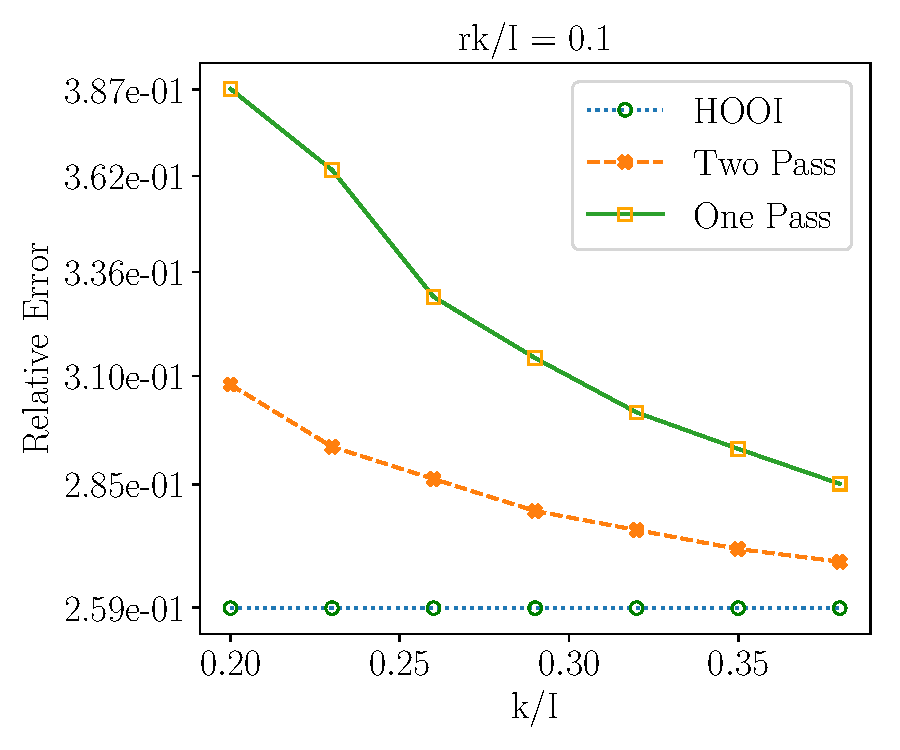
\includegraphics[scale = 0.29]{figure/ABSORB_frk10.pdf}
    \begin{subfigure}{0.31\textwidth}
    \end{subfigure}
    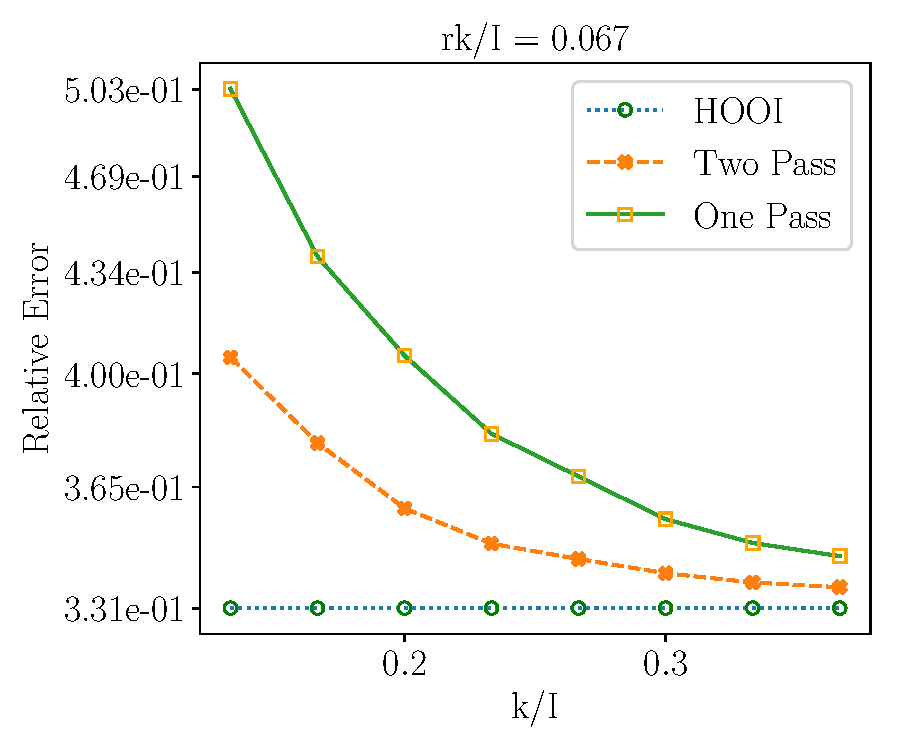
\includegraphics[scale = 0.29]{figure/ABSORB_frk15.pdf}
    \textbf{Aerosol Absorption}
\caption{Relative error for fixed-rank tensor approximation on climate simulation data ($240 \times 30 \times 192 \times 288$): \textit{We compared the relative errors presented in log scale for two-pass sketching, one-pass sketching and Tucker decomposition with different ranks ($rk/I = 0.125,0.2,0.067$).}} \label{fig:application}
\end{figure}
